% 概率公理 1 的示意图：样本空间 S 里的一个事件 E（仿 CME 106 速查表的插图）
\documentclass[tikz,dvisvgm,border=6pt]{standalone}
\definecolor{edge}{HTML}{E0624F}
\definecolor{face}{HTML}{F5CFC8}
\begin{document}
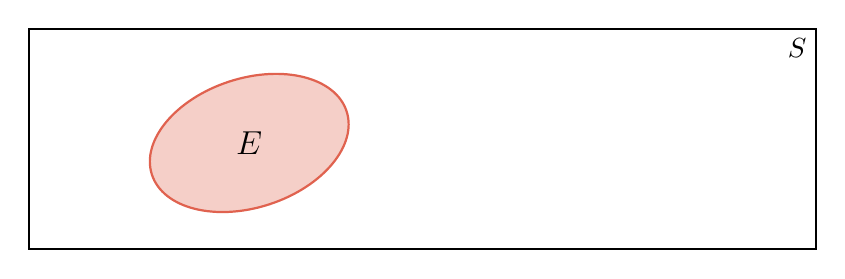
\begin{tikzpicture}
  \draw[thick] (0,0) rectangle (10,2.8);
  \node[anchor=north east] at (10,2.8) {$S$};
  \filldraw[draw=edge, fill=face, thick, rotate around={18:(2.8,1.35)}] (2.8,1.35) ellipse (1.3 and 0.82);
  \node at (2.8,1.35) {\large $E$};
\end{tikzpicture}
\end{document}
